\chapter{Sound \& Light}

\section{Miscellaneous}

\[
	\text{\% error} = \frac{\text{observed} - \text{theoretical}}{\text{theoretical}} * 100\%
\]

\section{Kinematics}

\[
	x = \frac{a}{2}(\Delta t)^2 + v_0\Delta t + x_0 \qquad
	v = v_0 + a\Delta t
\]\[
	v^2 = v_0^2 + 2a\Delta x \qquad
	\Delta x = \frac{v_0 + v}{2} * \Delta t
\]

\section{Simple Harmonic Motion}

\[
	x = A \cos(\omega t + \varphi) \quad
	v = -\omega A \cos(\omega t + \varphi) \quad
	a = -\omega^2 A \cos(\omega t + \varphi)
\]
\[
	x_{\max} = A \qquad
	v_{\max} = \omega A \qquad
	a_{\max} = \omega^2 A \qquad
	F_{\max} = m\omega^2 A
\]

\subsection{Springs and Slinkies}

$x$ represents the distance from the equilibrium.

If you put a mass on top of the slinky, $\Delta x_\text{eq}$ represents the difference between the original equilibrium and the new equilibrium.

\[
	F_s = kx = ma \qquad
	F_{s_{\max}} = k\Delta x_\text{eq} = 9.8 \Delta m
\]
\[
	f = \frac{1}{2\pi}\sqrt{\frac{k}{m}} \qquad 
	T = 2\pi\sqrt{\frac{m}{k}} \qquad 
	\omega = 2\pi f = \sqrt{\frac{k}{m}}
\]
\[
	SPE = \frac{1}{2} kx^2 \qquad
	KE = \frac{1}{2} mv^2
\]
\[
	TME = \frac{1}{2} kx^2 + \frac{1}{2} mv^2 = \frac{1}{2} kA^2 = \frac{1}{2} mv_{\max}^2
\]

\subsection{Springs in parallel and series}

% Converted from https://en.wikipedia.org/wiki/Series_and_parallel_springs using https://mediawiki2latex.wmflabs.org/

\begin{tabular}{|>{\RaggedRight}p{0.38225\linewidth}|>{\RaggedRight}p{0.23286\linewidth}|>{\RaggedRight}p{0.23286\linewidth}|} \hline 
	{\bfseries \hspace*{0pt}\ignorespaces{}\hspace*{0pt}Quantity}&{\bfseries \hspace*{0pt}\ignorespaces{}\hspace*{0pt}In Series}&{\bfseries \hspace*{0pt}\ignorespaces{}\hspace*{0pt}In Parallel} %\endhead  
	% \\ \hline \multicolumn{4}{|>{\RaggedRight}p{0.97143\linewidth}|}{\hspace*{0pt}\ignorespaces{}\hspace*{0pt}}
	\\ \hline \hspace*{0pt}\ignorespaces{}\hspace*{0pt}Equivalent spring constant&\hspace*{0pt}\ignorespaces{}\hspace*{0pt}{${\displaystyle {\frac {1}{k_{\mathrm {eq} }}}={\frac {1}{k_{1}}}+{\frac {1}{k_{2}}}}$}&\hspace*{0pt}\ignorespaces{}\hspace*{0pt}{${\displaystyle k_{\mathrm {eq} }=k_{1}+k_{2}}$}
	% \\ \hline \hspace*{0pt}\ignorespaces{}\hspace*{0pt}Equivalent compliance&\hspace*{0pt}\ignorespaces{}\hspace*{0pt}{${\displaystyle c_{\mathrm {eq} }=c_{1}+c_{2}}$}&\hspace*{0pt}\ignorespaces{}\hspace*{0pt}{${\displaystyle {\frac {1}{c_{\mathrm {eq} }}}={\frac {1}{c_{1}}}+{\frac {1}{c_{2}}}}$}
	\\ \hline \hspace*{0pt}\ignorespaces{}\hspace*{0pt}Deflection (elongation)&\hspace*{0pt}\ignorespaces{}\hspace*{0pt}{\itshape {${\displaystyle x_{\mathrm {eq} }=x_{1}+x_{2}}$}}&\hspace*{0pt}\ignorespaces{}\hspace*{0pt}{\itshape {${\displaystyle x_{\mathrm {eq} }=x_{1}=x_{2}}$}}
	\\ \hline \hspace*{0pt}\ignorespaces{}\hspace*{0pt}Force&\hspace*{0pt}\ignorespaces{}\hspace*{0pt}{${\displaystyle F_{\mathrm {eq} }=F_{1}=F_{2}}$}&\hspace*{0pt}\ignorespaces{}\hspace*{0pt}{${\displaystyle F_{\mathrm {eq} }=F_{1}+F_{2}}$}
	\\ \hline \hspace*{0pt}\ignorespaces{}\hspace*{0pt}Stored energy&\hspace*{0pt}\ignorespaces{}\hspace*{0pt}{${\displaystyle E_{\mathrm {eq} }=E_{1}+E_{2}}$}&\hspace*{0pt}\ignorespaces{}\hspace*{0pt}{${\displaystyle E_{\mathrm {eq} }=E_{1}+E_{2}}$}\\ \hline 
\end{tabular}

\subsection{Pendulums}

\[
	f = \frac{1}{2\pi}\sqrt{\frac{g}{L}} \qquad 
	T = 2\pi \sqrt{\frac{L}{g}}
\]

\section{Waves}

\[
	T = \frac{1}{f} \qquad
	v = \lambda f \qquad
	v = \frac{\Delta x}{\Delta t}
\]

\subsection{Slinkies and strings with fixed ends}

\[
	F_T = F_s = kx \qquad
	\mu = \frac{m}{L} \qquad
	v = \sqrt{\frac{F_T}{\mu}}
\]

Given mass $m_T$ hanging below a pulley, $F_T = m_T g$.

% \columnbreak

\section{Standing waves}

\subsection{Open-open, closed-closed}

$n$ is the number of antinodes, or the $n^\text{th}$ harmonic.

\[
	f_n = f_1 n = \frac{nv}{2L} \qquad f_1 = \frac{v}{2L} \qquad \lambda_n = \frac{2L}{n}
\]

\subsection{Open-closed}

\[
	f_n = f_1 n = \frac{nv}{4L} \qquad f_1 = \frac{v}{4L} \qquad \lambda_n = \frac{2L}{n}
\]

% \subsection{End correction}

% Although a theoretical air column will have a frequency only dependent on the velocity and length of the column, the diameter of the air column plays an effect in the real world.

% In an open-open pipe with diameter $d$:

% \[
% 	f_1 = \frac{v}{2(L + 0.6d)} \qquad \lambda_n = \frac{2(L + 0.6d)}{n}
% \]

% In an open-closed pipe with diameter $d$:

% \[
% 	f_1 = \frac{v}{4(L + 0.6d)} \qquad \lambda_n = \frac{4(L + 0.6d)}{n}
% \]
% \columnbreak

\section{Sound}

\subsection{Speed of sound}

\[
	v = 331 \sqrt{\frac{T_{\text{°C}}+273}{273}} \qquad v \approx 331 + 0.59T
\]

\subsection{Sound intensity}

\[
	I = \frac{\text{Power (\watt)}}{\text{Area}} = \frac{\text{Power (\watt)}}{4 \pi r^2} \qquad
\]

\[
	I_\decibel = 10 \log_{10} (\frac{I}{10^{-12}}) \qquad
	I = 10^{\frac{I_\decibel}{10} - 12}
\]

\subsection{Doppler effect}

\[\begin{aligned}
	\boxed{O}\smash{\rightarrow} \enspace \boxed{S} \quad f_o &= f_s \frac{v + v_o}{v} &
	\smash{\leftarrow}\boxed{O} \enspace \boxed{S} \quad f_o &= f_s \frac{v - v_o}{v}
	\\
	\boxed{O} \enspace \smash{\leftarrow}\boxed{S}  \quad f_o &= f_s \frac{v}{v - v_s} &
	\boxed{O} \enspace \boxed{S}\smash{\rightarrow} \quad f_o &= f_s \frac{v}{v + v_s}
	\\
	\boxed{O}\smash{\rightarrow} \enspace \smash{\leftarrow}\boxed{S} \quad f_o &= f_s \frac{v + v_o}{v - v_s} &
	\boxed{O}\smash{\rightarrow} \enspace \boxed{S}\smash{\rightarrow} \quad f_o &= f_s \frac{v + v_o}{v + v_s}
	\\
	\smash{\leftarrow}\boxed{O} \enspace \smash{\leftarrow}\boxed{S} \quad f_o &= f_s \frac{v - v_o}{v - v_s} &
	\smash{\leftarrow}\boxed{O} \enspace \boxed{S}\smash{\rightarrow} \quad f_o &= f_s \frac{v - v_o}{v + v_s}
\end{aligned}\]

\subsection{Constructive and Destructive Interference (2 dimensions)}

For a point on the $m^\text{th}$ antinodal/nodal line playing the same frequency with the same phase:

\[
	PD = m \lambda
\]

where $PD$ is the path length difference.

\subsection{Beats}

\[
	f_B = \Delta f
\]
% \columnbreak
\pagebreak
\section{Light}

\subsection{Speed of light}

\[
	c = 299\ 792\ 458 \frac{\metre}{\second} \approx 3 * 10^8 \frac{\metre}{\second}
\]

\subsection{Two-slit experiment}

\includegraphics[width=75mm]{content/soundlight/twoSlit}

\[
	PD = \frac{dy}{L} = m\lambda
\]

\subsection{Mirror}

\newcolumntype{L}{>{$}l<{$}} % math-mode version of "l" column type
\newcolumntype{R}{>{$}r<{$}} % math-mode version of "r" column type

% \begin{center}
% \begin{tabular}{R l L | L L L} 
% 	% \hline
% 	 & \text{Meaning} & & *) & *| & *( \\ 
% 	\hline
% 	r   & radius                     & m & + & \inf & - \\
% 	f   & focal length               & m & + & \inf & - \\
% 	p   & object distance            & m & + & + & +\\
% 	q   & image distance             & m & \pm & - & - \\
% 	h_o & object height   			 & m & + & + & + \\
% 	h_i & image height    			 & m & \pm & - & -  \\
% 	M   & magnification & \frac{m}{m}& \pm & - & - \\
% 	% \hline
% \end{tabular}
% \end{center}

\[
	r = 2f \qquad
	\frac{1}{f} = \frac{1}{p} + \frac{1}{q} \qquad
	M = \frac{h}{h_o} = \frac{-q}{p}
\]

In a plane mirror, $p = -q$.

\subsection{Lenses}

% converging () with wider middle $\Rightarrow$ positive focal length, diverging )( with thinner middle $\Rightarrow$ negative focal length.

\[
	\frac{1}{f} = (n-1)(\frac{1}{r_1} - \frac{1}{r_2}) \qquad
	\frac{1}{f} = \frac{1}{p} + \frac{1}{q} \qquad
	M = \frac{h}{h_o} = \frac{-q}{p}
\]

\subsubsection{Multiple lenses}

\[
	p_2 = \Delta x - q_1
\]

\subsection{Mirrors and Lenses}

% \begin{center}
% \begin{tabular}{R l L | L L L} 
% 	% \hline
% 		& \text{Meaning} & & *) & *| & *( \\ 
% 	\hline
% 	r   & radius                     & m & + & \inf & - \\
% 	f   & focal length               & m & + & \inf & - \\
% 	p   & object distance            & m & + & + & +\\
% 	q   & image distance             & m & \pm & - & - \\
% 	h_o & object height   			 & m & + & + & + \\
% 	h_i & image height    			 & m & \pm & - & -  \\
% 	M   & magnification & \frac{m}{m}& \pm & - & - \\
% 	% \hline
% \end{tabular}
% \end{center}

Real $\iff$ inverted, virtual $\iff$ upright.

\begin{center}
	\begin{tabular}{r | l l} 
		 & Converging & Diverging \\
		\hline
		Mirror & \includegraphics[width=2cm]{content/soundlight/ConvergingMirror.jpg} & \includegraphics[width=2cm]{content/soundlight/DivergingMirror.jpg} \\
		Lens & 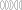
\includegraphics[width=2.25cm]{content/soundlight/ConvergingLenses.pdf} & 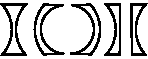
\includegraphics[width=2.5cm]{content/soundlight/DivergingLenses.pdf} \\
		focal length & + & - \\
		\hline
		object distance & image & image \\
		\hline
		$\infty$ to $2f$ & Real smaller & Virtual smaller \\
		$2f$ to $f$ & Real larger & \\
		$f$ to $0$ & Virtual larger & \\
		\hline
		$0$ to $-f$ & Virtual smaller & Virtual larger \\
		$-f$ to $-2f$ & & Real larger \\
		$-2f$ to $-\infty$ & & Real smaller \\
	\end{tabular}
\end{center}

\subsection{Refraction / Snell's Law}

The \textbf{normal line} is the line perpendicular to the surface which touches the intersection of the surface and the light ray.

The \textbf{incident angle} is the angle between the ray of light and the normal line.

$\theta_1$ and $\theta_2$ are both measured from the normal line, not the surface.

% The \textbf{index of refraction} ($n$, $\frac{\metre / \second}{\metre / \second}$) is the ratio of the speed of light in a vacuum over the speed of light in the medium.
Refraction occurs when the speed of light in two media are different and light hits the boundary of the two media. The frequency of the light will stay the same, but the speed, wavelength, and direction will change.
\[
	n = \frac{c}{v} \qquad n_1 \sin \theta_1 = n_2 \sin \theta_2
\]

\subsection{Ray diagrams}


